\documentclass{article}
    \usepackage{amssymb}
    \usepackage[utf8]{inputenc}
    \usepackage[russian]{babel}
    \usepackage[left=2cm,right=2cm,
        top=2cm,bottom=2cm,bindingoffset=0cm]{geometry}
    \usepackage{hyperref}
    \hypersetup{
        colorlinks=true,
        linkcolor=blue,
        filecolor=magenta,      
        urlcolor=cyan,
    }
  \usepackage{graphicx}
  \graphicspath{{pictures/}}
  \DeclareGraphicsExtensions{.pdf,.png,.jpg}
\usepackage{subcaption}
%\captionsetup{compatibility=false}

\begin{document}
\begin{center}{\hugeОтчет по курсовой работе за неделю\\}\end{center}
Дата: 5.11.2020\\
Научные руководители: Герасимов С.В., Мещеряков А.В.\\
Студент: Немешаева Алиса\\
Курс: 4\\

\renewcommand{\labelitemi}{$\blacksquare$}
\renewcommand\labelitemii{$\square$}
\begin{enumerate}
    \item Построены карты сегментации для Coma Cluster с помощью последних лучших моделей\\
        \begin{figure}[h]

            \begin{subfigure}{0.5\textwidth}
                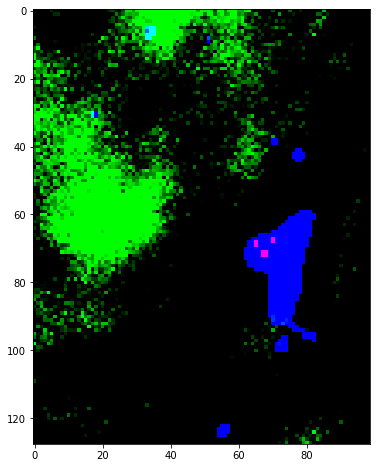
\includegraphics[width=0.7\linewidth]{pz_act_coma} 
                \caption{Для модели обученной на каталоге planck\_z}
            \end{subfigure}
            \begin{subfigure}{0.5\textwidth}
                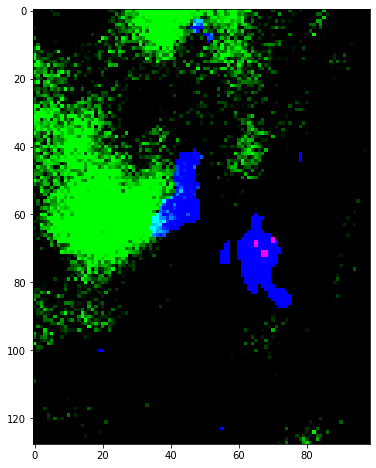
\includegraphics[width=0.7\linewidth]{pz_coma}
                \caption{Для модели обученной на каталоге planck\_z+act}
            \end{subfigure}

        \caption{Маска скопления для Coma Cluster синим цветом}
        \end{figure}
    \item Может показаться, что стоит рассмотреть параметр площади пятна скопления на маске 
        сегментации. Но этот параметр не позволяет разделить каталог по степени уверенности в 
        объектах.\\
        \begin{figure}[h]
            \center{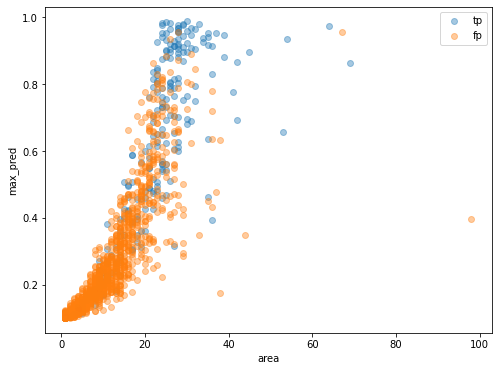
\includegraphics[width=0.7\linewidth]{act_model_area_pred_ind}}
        \caption{Зависимость объектов каталога по параметрам area и max\_pred}
        \end{figure}

    \item На этой неделе была написана базовая часть статьи о полученных каталогах по данным 
        planck\_z и planck\_z+act. Для написания вводной части использовались некотрые статьи, 
        далее приведены ссылки на них и выжимки из введений:\\
\end{enumerate}
\section{Clusters and superclusters in the Sloan Digital Sky Survey}
\hyperlink{https://www.aanda.org/articles/aa/pdf/2003/26/aah4162.pdf}{Статья}\\

Скопления и группы галактик - это базовые блоки, из которых строится Вселенная на космолгическом 
уровне.\\

Некоторые каталоги скоплений и групп галактик были созданы с помощью каталогов галактик. Аналогичным 
образом на более высоких уровнях иерархии каталоги сверхскоплений были созданы из каталогов скоплений.\\

Цель этой статьи - построить карту Вселенной вплоть до красного смещения z=0.2.\\

Авторы статьи вычисляют поле плотности данных SDSS для нахождения скоплений и сверхскоплений галактик,
а также для изучения их характеристик.\\

Скопления определяются как увеличения значения поля плотности. Для отделения скоплений с различными
параметрами размера и светимости используются различные параметры сглаживания. Для нахождения 
скоплений и групп галактик используется поле плотности с высоким разрешением, а для сверхскоплений 
- поле плотности с низким разрешением.\\ 

Авторы статьи исследуют скопления и сверхскопления как объекты, выявляющие структуру локальной 
Вселенной.\\

Использование метода плотности поля может выявить новые, прежде незафиксированные скопления (в 
особенности скопления с малым количеством галактик), и в таком случае будет получена более точная 
картина распределения скоплений в пространстве. Однако некоторые из таких скоплений могут быть 
динамически нестабильными, и обнаруженная информация может отражать лишь ситуацию в развитии 
скопления на данный момент.\\

\section{Towards understanding the structure of voids in the cosmic web}
\hyperlink{https://www.aanda.org/articles/aa/pdf/2011/10/aa17248-11.pdf}{Статья}

Цель этой серии статей - изучить роль возмущений на различных масштабах в формировании структуры 
Вселенной.\\

Сверхскопления - это объекты, для которых волны средних и больших масштабов накладываются в 
соответствующих фазах для формирования пиков высокой плотности. Аналогично, войды - это области 
пространства, где возмущения плотности средних и больших масштабов накладываются в соответствующих 
фазах низкой плотности.\\

Параметры космической паутину значительно зависят от возмущений малых и средних масштабов, в то время 
как возмущения больших масштабов влияют на насыщенность скоплений галактиками, а также на наполненность
войдов. Это исследование посвящено волнам средних и больших масштабов.\\

Скопления галактик не распределены случайно, но формирут нити, которые в пересечении содержат 
сверхскопления. Пространство между нитями почти не содержит галактики и формирует войды.\\

Судя по вытянутой форме нитей, галактики и группы галактик были сформированы одновременно с 
формированием космической паутины.\\

Судя по симуляциям тёмной материи, войды должны содержать редкие галактики, но в реальности это не 
так.\\

\section{PSZSPT: a joint Planck and SPT-SZ cluster catalogue}
\hyperlink{https://arxiv.org/pdf/2009.08822.pdf}{Статья}

Скопления галактик представляют собой уникальные объекты для изучения образования структуры 
Вселенной. С их помощью также можно улучшить понимание образования структуры и эволюции галактик. 
Для изучения скоплений с астрофизической и космологической точки зрения нужно двугаться в двух 
направлениях: увеличение количества известных скоплений и лучшее понимание их свойств. Изучение 
многоканальных данных обязательно для достижения этих целей.\\

Для извлечения скоплений используются гибридные методы: рентгеновские и микроволновые каталоги 
уточняются с помощью оптических данных. Другой способ поиска скоплений - детектировать их на 
нескольких диапазонах одновременно. Кроме того, получать более качественные каталоги скоплений 
можно при объединении данных разных обзоров одного диапазона.\\

Данная статья фокусируется на совместном исследовании данных Planck и SPT-SZ с помощью Matched 
Multi Filter.\\

\section{Superclusters of galaxies from the 2dF redshift survey}
\hyperlink{https://www.aanda.org/articles/aa/pdf/2007/05/aa5296-06.pdf}{Статья}

Галактики образуют различные системы от групп и скоплений до сверхскоплений. Системы галактик 
не расположены в пространстве случайным образом: группы и скопления в основном выровнены по 
цепочкам (нитям), а пространство между группами заполнено галактиками вдоль цепочки. Самые большие
системы галактик - это сверхскопления галактик, которые содержат скопления и группы галактик с 
окружающими их нитями галактик.\\

Сверхскопления галактик используются для широкого круга исследований. Сверхскопления создаются
крупномасштабными возмущениями плотности, которые развиваются очень медленно. Таким образом, 
распределение сверхскоплений содержит информацию о крупномасштабном начальном поле плотности, и их 
свойства можно использовать для проверки различных космологических моделей. Внутренняя структура
сверхскоплений сохраняет информацию о формировании и эволюции галактик на средних масштабах. 
Свойства галактик и групп в различных средах сверхскоплений можно использовать для изучения 
эволюции галактик в малых масштабах.\\

Основная цель этой статьи - составить новый каталог сверхскоплений с использованием 2dFGRS.\\

\section{Planck 2015 results}
\hyperlink{https://www.aanda.org/articles/aa/pdf/2016/10/aa25823-15.pdf}{Статья}

Пики в космологическом поле плотности схлопываются и сливаются, образуя гравитационно связанные 
гало с возрастающей массой. Скопления галактик являются наиболее массивными из этих связанных 
структур и указывают на экстремумы космологического поля плотности на соответствующих масштабах.
Таким образом, эволюция обилия скоплений галактик с изменением массы и красного смещения является
чувствительным космологическим исследованием Вселенной позднего времени.\\

Скопления галактик - это многокомпонентные объекты, состоящие из темной материи (которая 
преобладает в массе), звезд, холодного газа и пыли в галактиках, а также горячей ионизированной
внутрикластерной среды (ICM). Эти различные компоненты делают кластеры истинными многоволновыми 
объектами. Галактики излучают в оптическом и инфракрасном диапазоне. ICM, который составляет 
большую часть барионного материала по массе, излучает в рентгеновских лучах посредством теплового
тормозного излучения и линейного излучения и увеличивает энергию фотонов космического микроволнового 
фона (CMB) посредством обратного комптоновского рассеяния.\\

\section{The Atacama Cosmology Telescope: A Catalog of > 4000 Sunyaev-Zel’dovich Galaxy Clusters}
\hyperlink{https://arxiv.org/pdf/2009.11043.pdf}{Статья}

Амплитуда эффекта Сюняева-Зельдовича изменяется в зависимости от массы скопления. В этой статье 
авторы представляют новый каталог, извлченный из данных ACT с помощью Advanced ACTPol reciever.\\

Отчет согласован с научным руководителем.\\
Общее количество строк кода за эту неделю: 76\\
\hyperlink{https://github.com/rt2122/data-segmentation-2}{Репозиторий}\\ 
\end{document}
